\chapter{Introduction} \label{chp:Introduction}

 In this work we want to tackle a specific algorithmic problem: Navigating a swarm of particles to a goal position in a maze-like environment, by applying a global uniform force. This problem finds its application in medicine in form of targeted drug delivery. The goal is to localize medical treatment to efficiently combat cancer, localized infections or internal bleeding, without causing unwanted and potentially harmful side effects for the rest of the body. The delivery requires careful navigation of the distributed microscopic particles through pathways of blood vessels to a target location. As the particles are too small to build microrobots with sufficient energy to swim against flowing blood, a global external force like an electromagnetic field is used for motion control. This means all particles are subjected into the same direction unless their path is blocked by obstacles. Since all the particles start in different locations, navigating all particles by a uniform force to a single destination is notoriously hard. Figure \ref{fig:brain_tumor} gives an example for an abstract view on the problem.

 \begin{figure}[ht]
    
    \begin{center}
        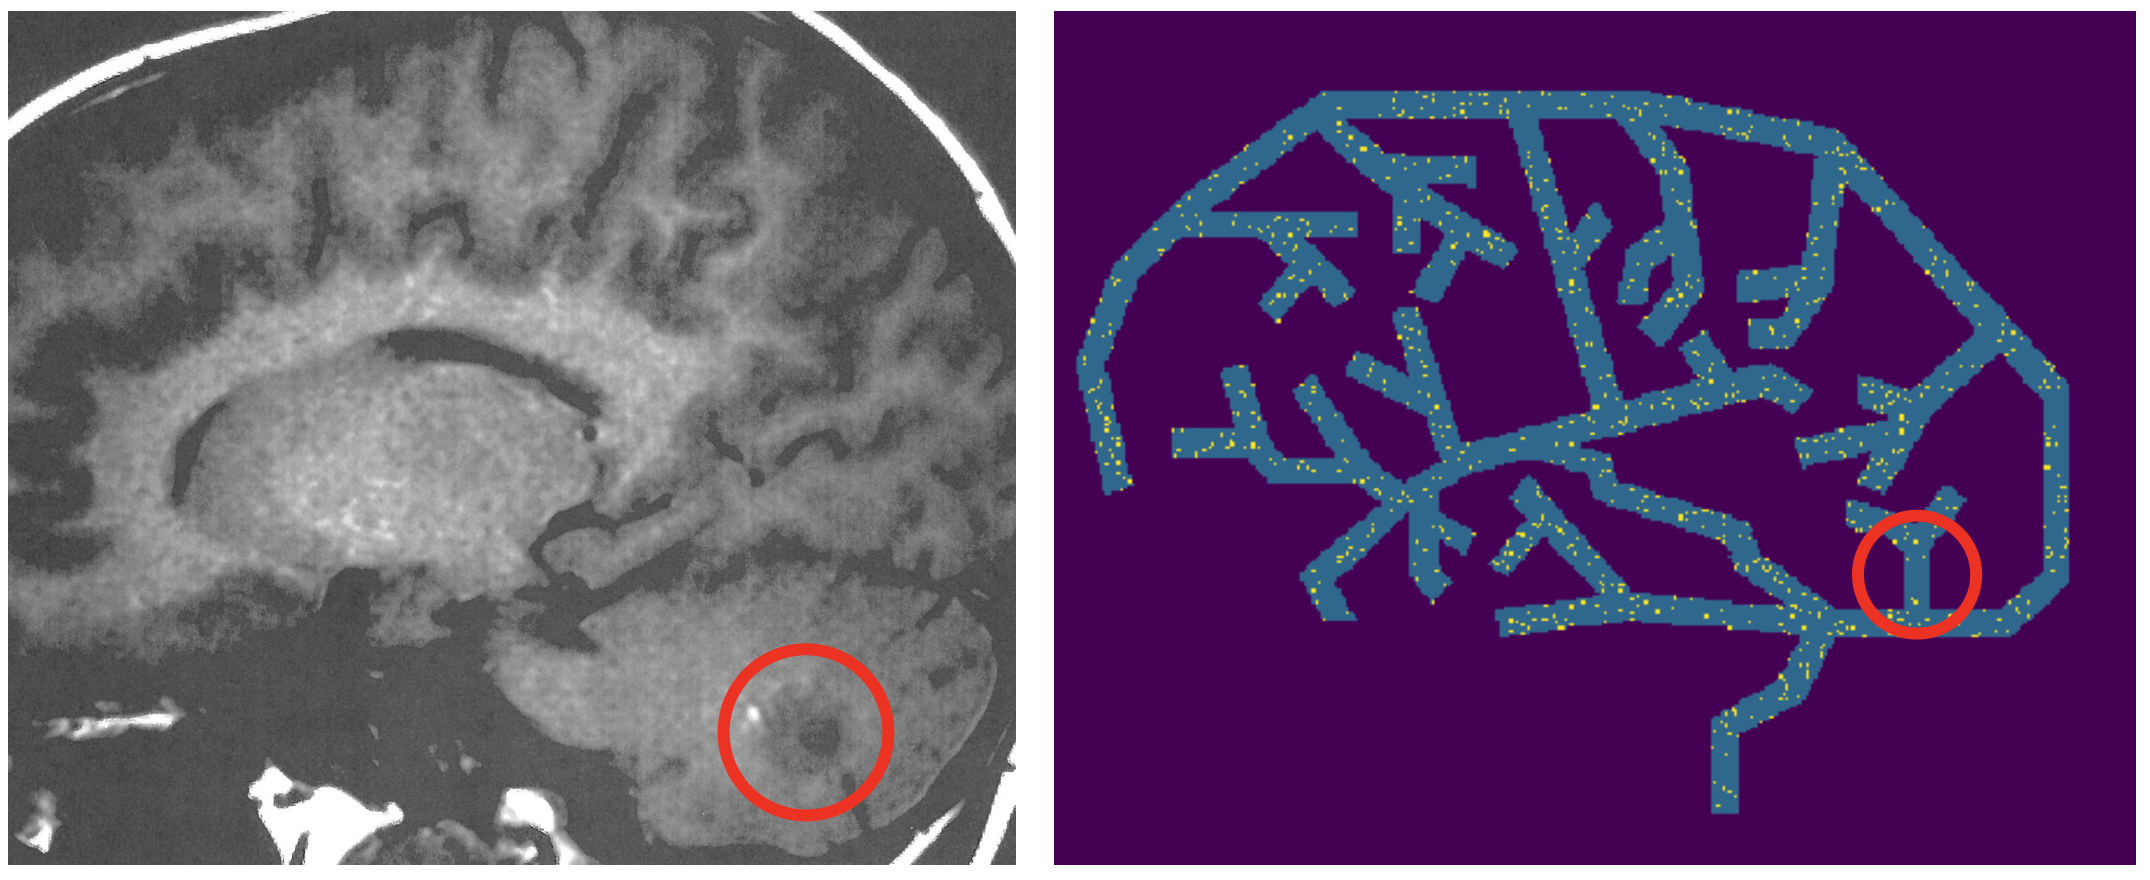
\includegraphics[clip, width=0.7\columnwidth]{figures/drugdelivery/brains.png}
    \end{center}
    
    %\vspace*{-6pt}
    \caption[Targeted Drug Delivery Motivation]{Targeted drug delivery for tumor treatment (from \cite{becker2020}). An MRI image on the right shows a tumor (marked by the red circle) and an abstracted version (left) shows particles containing some sort of medicine (yellow dots) which should be delivered to the target region.}
    \label{fig:brain_tumor}
    %\vspace*{-12pt}
\end{figure}

In 2020 it was proven by Becker et al. \cite{becker2020} that the navigation problem itself is NP-hard. This means, that approximation algorithms will be very important for any practical application. Becker et al. also showed, that it is possible to solve certain instances of the problem using reinforcement learning (RL) and that the resulting solution outperformed current approximation algorithms. While their approach delivered a proof-of-concept, it was computationally very heavy compared to the algorithmic approaches, as the RL algorithm needed millions of training steps before it could solve the problem. 
 
 Building up on this previous work, we want to improve the process of how RL algorithms can be used to solve this problem. Our goal is to speed up the learning process, train agents which generalize for multiple instances and investigate the possibilities of reinforcement learning to deal with extended settings which are closer to real-world targeted drug delivery. Our results may also be useful for the application of reinforcement learning on other algorithmic problems.

 \paragraph{Learning by Doing: Reinforcement Learning} 
In this work we will be using techniques from a specific field of machine learning called reinforcement learning or more specifically its modern combination with artificial neural networks called \textit{deep reinforcement learning}.

 Deep reinforcement learning is one of the most exciting fields of machine learning today, because it is capable of achieving actual superhuman performance without any human ever creating training data for it. In reinforcement learning the data is created solely by an agent interacting with its environment -- similar to how humans learn by trail and error. Deep reinforcement learning algorithms therefore are unsupervised machine learning algorithms.

 Like traditional machine learning, reinforcement learning has been around for decades, but just recently gained notable attention. In 2013 researchers from the British startup DeepMind were able to train a system to play any game from the game console Atari without prior knowledge and only with raw pixel data as input \cite{mnih2013playing}. They later even improved their system and were able to outperform trained human players \cite{mnih2015human}.These two successes were the beginning of a series of advances for deep reinforcement learning. In 2016 a team from Google DeepMind created a RL agent called \textit{AlphaGo} which was able to defeat multiple worlds top class Go players including the 2017 world champion Ke Jie \cite{borowiec2016alphago}. The system was later expanded to also play Shogi and Chess and renamed to \textit{AlphaGo Zero}. This new system gained notable attention, as it was able to defeated the state-of-the-art alpha-beta search engine for chess Stockfish \cite{silver2017mastering}. In 2019 they reached a new milestone, when their system \textit{AlphaStar} was able to beat a professional player at StarCraft II -- a complex multiplayer strategy game \cite{arulkumaran2019alphastar}. 

 All these advances were made possible by a number of breakthroughs in machine learning and reinforcement learning as well as an increase in computational power over the last decade. The victory of AlphaGo Zero over its algorithmic competitor Stockfish also demonstrates how RL algorithms can be used as a replacement for algorithmic solutions in completely new areas of computer science. 


\section{Previous and Related Work} \label{sec:RelatedWork}
In this thesis, we want to use reinforcement learning to train neural networks to steer large numbers of microrobots or microscopic particles through a maze-like environment to a goal position. In a real-world scenario this maze-like environment may be the blood vessels in a human body, and the target position may be a tumor. 

To date, we already have the possibility to create particles which contain a magnetic core and have a catalytic or biodegradable surface which allows them to release their payload at the target position \cite{litvinov2012high, mellal2015magnetic}. To navigate these particles through the blood vessels, magnetic fields produced by modified gradient coils inside of an MRI scanner can be used \cite{mathieu2007magnetic, mathieu2010steering}. The scanner can also be used to provide real-time feedback and track the position of the nanoparticles \cite{pouponneau2009magnetic}. Since blood vessels build a complex system of paths, directing the particles to the goal position requires efficient motion planning algorithms. 

Controlling a larger number of particles by global inputs has been studied in very different settings in the past. Assembling complex shapes using a swarm of particles was explored in \cite{becker2018tilt} and \cite{balanza2019full}. Often it is not required to bring the particles to a goal position, but to rearrange them in a certain way, which has been done in \cite{becker2013massive} and \cite{zhang2017rearranging}. 

Moving particles to a goal position is directly related to another problem studied in the past called \textit{rendezvous search} \cite{alpern2006theory}. Rendezvous search aims at finding a sequence of movements for two or more independent agents to meet at the same location. Since it is easy to move a single particle (or a number of particles concentrated at a single point) to the goal position via the shortest available path, we can express our problem by a sequence of rendezvous between particles, ultimately gathering all particles at a single location.

 Early algorithmic approaches and settings were introduced by Alpern and Gal \cite{alpern2006theory} as well as by Anderson and Fekete \cite{anderson2001two}. Their work included agents with limited onboard computations, but in certain cases both agents followed the same movement protocol -- executing the same movement. The problem can therefore also be called \textit{symmetric} rendezvous search where the symmetry is only broken by interaction with obstacles. Since all agents perform the same movements, this directly corresponds to the particle navigation problem. 

Rendezvous search was extended into a sequence of rendezvous to collect a swarm of particles in a single place by Mahadev et al. \cite{mahadev2016collecting}. Just recently it was proven, that computation of an optimal gathering sequence is NP-hard \cite{becker2020}. The authors also proposed several new approximation algorithms, including an approach for the application of reinforcement learning \cite{huang2019, becker2020}. Even though the reinforcement learning approach is computationally more expensive, it produces much shorter gathering sequences.

In their approach, Becker et al. used recent techniques to train the RL agent. To improve training, they included an intrinsic reward signal, guiding the agent to explore "interesting" environment states. This technique was explored for a long time to supplement sparse extrinsic rewards \cite{pathak2017curiosity, mohamed2015variational, houthooft2016variational} and recently found notable attention with the introduction of the \textit{intrinsic curiosity module} \cite{burda2018large} and the \textit{random network distillation} methods \cite{burda2018exploration}. The latter uses prediction error to simulate real intrinsic motivation. Both techniques have shown to drastically improve performance on "hard" games from the Atari game suite when used in combination with the well-known trust region optimization technique \textit{proximal policy optimization} \cite{schulman2017proximal}. Just recently, Baida et al. presented an improved curiosity signal which has shown to work exceptionally well even in the presence of extremely noise maze-like environments \cite{badia2020never}.

\section{Our Results} \label{sec:Results}
To evaluate reinforcement learning (RL) algorithms, we implemented a laboratory environment for RL agents called Baselines Lab. We also implemented a high-performance simulation for the particle navigation problem. Using these two components in a series of experiments, we provide a number of insights on improving the performance of RL agents on the distributed particle navigation problem:

\begin{itemize}
    \item We provide a novel continuous reward to guide RL agents in environments with distributed particles which accelerates training (see Section \ref{sec:MazeReward} and Section \ref{sec:EvalReward}).
    \item We perform an extensive study on different rewards, including previous goal-based reward, our continuous reward and combinations with intrinsic curiosity reward (see Section \ref{sec:EvalReward}).
    \item We perform a study on the performance of different RL algorithms and provide a set of optimized hyperparameters for each of them (see Section \ref{sec:EvalRLAlgorithms}).
    \item We perform a study on observation preprocessing, including observation downscaling (see Section \ref{sec:Eval/ObsSize}) and frame stacking (see Section \ref{sec:EvalObs}).
    \item We analyze the impact of different structures for neural networks and used activation functions (see Section \ref{sec:Eval/NetworkStructure}).
    \item We provide a new baseline for the performance of RL agents together with a comparison with previous RL and algorithmic approaches (see Section \ref{sec:EvalBaseline}).  
\end{itemize}

\noindent Additionally, we studied the impact on training performance when introducing additional real-world problems:

\begin{itemize}
    \item We show that RL agents are capable of dealing with simplified physical particle behavior (see Section \ref{sec:EvalPhysical}).
    \item We show that RL agents are able to deal with a certain amount of observation error, including random noise and false positive and negative detection of particles (see Section \ref{sec:EvalError}).
    \item We show that RL agents are also able to deal with a certain amount of action error, including repeated (sticky) actions, partially random actions and actions which only affect a random number of particles. (see Section \ref{sec:EvalError}). 
\end{itemize}

\noindent Finally, we made advances in generalizing agent behavior for more than a single instance:

\begin{itemize}
    \item We show, that agents are able to learn strategies which can gather particles at random goal positions for a single maze instance (see Section \ref{sec:EvalRandomGoals}).
    \item We show that agents are able to learn strategies which can gather particles at random goal positions for multiple small instances (see Section \ref{sec:EvalRandomMaze}).
\end{itemize}
